\documentclass[tikz, border=2pt]{standalone}
\usepackage{graphicx} 
\usepackage{tikz} 
\usepackage{tikz-3dplot} 
\usetikzlibrary{angles,quotes,arrows.meta, positioning} 
\usepackage{pgfplots} 
\pgfplotsset{compat=1.18} % Pacchetti Matematici 
\usepackage{amsmath, amssymb, amsthm} 

\definecolor{myblue}{HTML}{139FE9}
\begin{document}
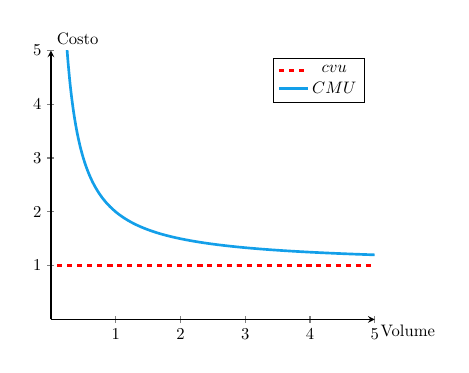
\begin{tikzpicture}[scale=0.6,
  declare function={
    f(\x) = 1 + 1/\x;
    g(\x) = 1;
}]
  \begin{axis}[
    xlabel={Volume}, ylabel={Costo},
    xmin=0, xmax=5, ymin=0, ymax=5,
    grid=none, axis lines=middle, 
    axis line style={-stealth, thick},
    tick style={thick},
    xlabel style={at={(ticklabel* cs:1)}, anchor=north west},
    ylabel style={at={(ticklabel* cs:1)}, anchor=south west},
    samples=100, unbounded coords=jump, legend pos=north east]
    \addplot[domain=0.1:5, dashed, ultra thick, smooth, color=red]{g(x)};
    \addplot[domain=0.1:5, ultra thick, smooth, color=myblue]{f(x)};
    \legend{$cvu$, $CMU$}
  \end{axis}
\end{tikzpicture}
\end{document}
